\documentclass{beamer}

% Beamer style stuff
\usetheme[style=plain]{uu}
% \setbeamertemplate{note page}[plain]

\usepackage{graphicx}
\usepackage{mathtools}
\usepackage{amssymb}
\usepackage{hyperref}
\usepackage{color}
\usepackage{float}

%% unicode support, for text and code :)
\usepackage[utf8x]{inputenc}
\usepackage{ucs}
\usepackage{autofe}


%% Haskell syntax highlighting and code font
\usepackage{minted}
\usepackage{fancyvrb}
\usepackage{inconsolata}
\usemintedstyle{default}

\newmint{haskell}{mathescape,fontfamily=tt,fontsize=\footnotesize}
\newmintedfile{haskell}{xleftmargin=20pt,mathescape,fontfamily=tt,fontsize=\footnotesize}
\newminted{haskell}{xleftmargin=20pt,gobble=12,mathescape,fontfamily=tt,fontsize=\footnotesize}

\newmint{coq}{mathescape,fontfamily=tt,fontsize=\footnotesize}
\newmintedfile{coq}{xleftmargin=20pt,mathescape,fontfamily=tt,fontsize=\footnotesize}
\newminted{coq}{xleftmargin=20pt,gobble=12,mathescape,fontfamily=tt,fontsize=\footnotesize}


%% Metainformation
%% PDF stuff
\usepackage{datetime}
\usepackage{ifpdf}
\ifpdf
\pdfinfo{
    /Author (Joao Paulo Pizani Flor)
    /Title (Comparing functional EDSLs for hardware description)
    /Keywords (Hardware verification, Functional Programming, Hardware design, Dependently-typed programming, Coq, Lava, ForSyDe, Haskell, Coquet)
    /CreationDate (D:\pdfdate)
}
\fi

\title[Comparing functional EDSLs for hardware description]{Comparing functional Embedded Domain-Specific Languages for hardware description}

\date{February 13th, 2014}

\author[Pizani Flor]
{
    João Paulo Pizani Flor
}

\institute[Utrecht University]
{
    Department of Information and Computing Sciences,
    Utrecht University
}

\subject{Function Programming, Hardware verification, Haskell, Coq, Lava, Coquet, ForSyDe}




\begin{document}

%% The document itself
    \begin{frame}
        \titlepage
    \end{frame}

    \begin{frame}
        \frametitle{Table of Contents}
        \tableofcontents
    \end{frame}


    \section{Introduction}
\label{sec:introduction}
    \frame{\sectionpage}

    \subsection{Hardware design}
    \label{subsec:hardware-design}
        \begin{frame}
            \frametitle{Hardware design}
        \end{frame}


    \subsection{Domain-Specific Languages}
    \label{subsec:domain-specific-languages}
        % deep-embedded / shallow embedded
        \begin{frame}
            \frametitle{Domain-Specific Languages}

            \par{A computer language (turing-complete or \emph{not}) targeting a \emph{specific application domain.}}
            \par{\textbf{Example DSLs:}}
            \begin{itemize}
                \item SQL (database queries)
                \item CSS (document formatting)
                \item MATLAB (Matrix programming)
                \item VHDL (Hardware description)
            \end{itemize}

            \pause

            \par{A DSL can also be \emph{embedded} in a general-purpose language.}
            \par{\textbf{Example EDSLs:}}
            \begin{itemize}
                \item Boost.Proto (C++ / parser combinators)
                \item Diagrams (Haskell / programmatic drawing)
                \item Parsec (Haskell / parser combinators)
            \end{itemize}
        \end{frame}

        \begin{frame}[fragile]
            \frametitle{Example of an EDSL: \texttt{Parsec}}

            A simple parser for a "Game of Life"-like input format:
            \haskellfile{code/parsec-example.hs}
\end{frame}


    \subsection{Hardware EDSLs}
    \label{subsec:hardware-edsls}
        \begin{frame}
            \frametitle{Hardware EDSLs}
            An EDSL used for hardware design-related tasks. Can encompass:

            \begin{itemize}
                \item Modeling / description
                \item Simulation (validation)
                \item Formal verification
                \item Synthesis to other (lower-level) languages
            \end{itemize}
        \end{frame}

        \begin{frame}
            \frametitle{Example of a hardware EDSL}

            Some Lava code\ldots
        \end{frame}

    \section{Analyzed EDSLs}
\label{sec:analyzed-edsls}
    \frame{\sectionpage}

    \begin{frame}
        \frametitle{Choice criteria}

        \par{When choosing which EDSLs to study, our requirements were:}
        \vspace{0.3cm}
        \begin{itemize}
            \item Hosted on already-known languages
            \item Covered a wide range in the criteria we defined (variety)
            \item Originals instead of variants or improvements
            \item Relatively well-known, frequently cited
        \end{itemize}
    \end{frame}


    \subsection{Chosen EDSLs}
    \label{subsec:chosen-edsls}
        \begin{frame}
            \frametitle{Chosen EDSLs}
            \par{The language we chose to evaluate, with the respective host language, were:}
            \vspace{0.3cm}
            \begin{itemize}
                \item Lava (Haskell - \texttt{chalmers-lava} variant)
                \item ForSyDe (Haskell)
                \item Coquet (Coq interactive theorem prover)
            \end{itemize}
        \end{frame}

    \subsection{Evaluation criteria}
    \label{subsec:evaluation-criteria}
        \begin{frame}
            \frametitle{Evaluation criteria}
            \par{As \emph{orthogonal} as possible:}
            \vspace{0.3cm}
            \begin{itemize}
                \item Simulation (validation)
                \item (Formal) verification
                \item Genericity (data, structure)
                \item Depth of embedding
                \item Tool integration
                \item Extensibility
            \end{itemize}
            \vspace{0.2cm}
            \par{Even though \emph{depth of embedding} can influence other criteria\ldots}

            \note{
                \begin{itemize}
                    \item Orthogonal means independent

                    \item Functional simulation (inputs/outputs)
                    \item Diff validation/verification:
                        \begin{itemize}
                            \item Did we build the thing right? (validation)
                            \item Did we build the right thing? (verification)
                        \end{itemize}
                    \item Generic or parameterized families of circuits
                        \begin{itemize}
                            \item I/O sizes
                            \item Other: \emph{iterations} in a crypto circuit, etc.
                        \end{itemize}
                    \item Depth of embedding: deep means datatype for circuits
                    \item Integration with other hardware tools: synthesis, timing, model checkers
                \end{itemize}
            }
        \end{frame}

    \section{Modeled circuits}
\label{sec:circuits}

    When thinking of which circuits to model using the analyzed EDSLs, some principles guided us.
    First of all, they shouldn't be too simple but also not too complex. Some very simple circuits
    (adders, counters, etc.) are very often shown as examples in the papers that define the EDSLs
    themselves, as well as in tutorials. On the other hand, we also did not want to model too
    complex circuits; that would require too much effort on the hardware design itself, and diverge
    from the focus of this project, which is to evaluate and analyze the EDSLs.

    Another principle that guided our choice is that the circuits should be immediately familiar to
    anyone with some minimal experience in hardware design. We avoided, therefore, considering
    application-specific circuits such as those for Digital Signal Processing (DSP), implementing
    communication protocols, etc. Having ruled out this class of circuits, we were left to choose
    from circuits that form a general-purpose computing machine, such as arithmetic units, memory
    blocks, control units and so forth.

    Finally, we wanted to choose among circuits that already had a well-defined, \emph{behavioural}
    description, to avoid using any of the analyzed EDSLs as ``basis'' of comparison.

    Taking these considerations into account, we chose to implement, in each of the EDSLs analyzed,
    three circuits originating from the book ``The Elements of Computing
    Systems''\cite{nand2tetris-book}. This book aims to give the reader a deep understanding of how
    computer systems work by taking a hands-on approach, in which the reader is given the most basic
    logic gates and builds, step-by-step, all the hardware and software components necessary to
    implement a complete computer system.

    From the hardware design part of the book, we took our three circuits to be modeled:

    \begin{itemize}
        \item A simple Arithmetic Logic Unit (ALU), from here onwards referred to as ``circuit 1''.

        \item A RAM memory block with 64 words, from here onwards referred to as ``circuit 2''.

        \item A CPU with an extremely reduced instruction set (capable of executing the \emph{Hack}
            assembly language defined in the book) from here onwards referred to as ``circuit 3''.
    \end{itemize}

    \subsection{Circuit 1: ALU}
    \label{subsec:circuit-alu}

        The Arithmetic Logic Unit built by us is a 2-input ALU, in which each of the inputs (as well
        as the output) is a 16-bit long word (interpreted as two's-complement signed integer). It is
        capable of computing several functions, and the choice of which function to compute is made
        by setting the ALU's 6 \emph{control bits}. To become more familiar with this circuit, let's
        first take a look at its block diagram, shown in figure \ref{fig:alu-block}

        \begin{figure}[h!]
            \centerline{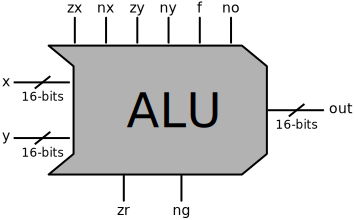
\includegraphics[width=0.5\textwidth]{imgs/alu-block.pdf}}
            \caption{Block diagram of circuit 1, showing its input and output ports.
                \label{fig:alu-block}}
        \end{figure}

        Each of the 6 control bits to the ALU has, in isolation, a well-defined effect on the inputs
        or outputs to the ALU core. The bits \texttt{(zx, nx, zy, ny)} control ``pre-processing''
        steps for the inputs \texttt{x} and \texttt{y}, with the following behaviour:

        \begin{description}
            \item[zx and zy] \emph{Zeroes} the x input (respectively y). The ALU core will receive
                \texttt{0} as input.

            \item[nx and ny] Performs \emph{bitwise negation} of input x (respectively y).
        \end{description}

        Therefore, the ALU ``core'' itself (adder, and gate) has, as inputs, the results of
        performing these pre-processing steps controlled by \texttt{(zx, nx, zy, ny)}.  Furthermore,
        the \emph{output} of the ALU core can also be \emph{bitwise negated} as a
        ``post-processing'' step, controlled by bit \texttt{no}.

        Finally, the control bit $f$ can be used to select which operation is to be performed by the
        ALU core: if we wish to add the two inputs, we need to set $f = 1$, and if we want bitwise
        conjunction, then we need to set $f = 0$.

        Besides the main (16-bit wide) output of the ALU, there are two other output \emph{flags},
        that indicate predicates over the main output:

        \begin{description}
            \item[zr] Is high whenever $out = 0$.
            \item[ng] Is high whenever $out < 0$.
        \end{description}

        When the ALU is used in the context of a microprocessor these flags can be used, for
        example, to facilitate conditional jumps.

        Even though there are $2^{6} = 64$ possible combinations for the values of the control bits,
        only 18 of these combinations result in interesting functions -- that is because several
        combinations of control bits can be used to calculate the same function. We show these 18
        functions that the ALU can calculate on table \ref{tab:alu-functions}.
        \begin{table}[h]
    \begin{center}
        \begin{tabular}{ccccccc}
            \toprule
            \textbf{zx} & \textbf{nx} & \textbf{zy} &
            \textbf{ny} & \textbf{f} & \textbf{no} & \textbf{out=}
            \tabularnewline
            \midrule

            1  &  0  &  1  &  0  &  1  &  0  &   $0$  \\

            1  &  1  &  1  &  1  &  1  &  1  &   $1$  \\

            1  &  1  &  1  &  0  &  1  &  1  &   $-1$  \\

            0  &  0  &  1  &  1  &  0  &  0  &   $x$  \\

            1  &  1  &  0  &  0  &  0  &  0  &   $y$  \\

            0  &  0  &  1  &  1  &  0  &  1  &   $\neg x$  \\

            1  &  1  &  0  &  0  &  0  &  1  &   $\neg y$  \\

            0  &  0  &  1  &  1  &  1  &  1  &   $-x$  \\

            1  &  1  &  0  &  0  &  1  &  1  &   $-y$  \\

            0  &  1  &  1  &  1  &  1  &  1  &   $x + 1$  \\

            1  &  1  &  0  &  1  &  1  &  1  &   $y + 1$  \\

            0  &  0  &  1  &  1  &  1  &  0  &   $x - 1$  \\

            1  &  1  &  0  &  0  &  1  &  0  &   $y - 1$  \\

            0  &  0  &  0  &  0  &  1  &  0  &   $x + y$  \\

            0  &  1  &  0  &  0  &  1  &  1  &   $x - y$  \\

            0  &  0  &  0  &  1  &  1  &  1  &   $y - x$  \\

            0  &  0  &  0  &  0  &  0  &  0  &   $x \wedge y$  \\

            0  &  1  &  0  &  1  &  0  &  1  &   $x \vee y$  \\

            \bottomrule
        \end{tabular}
    \end{center}
    \label{tab:alu-functions}
    \caption{Functions that the ALU can calculate, given different settings of the control bits}
\end{table}


        %% TODO: Talk about the construction of the ALU in terms of its parts.


    \subsection{Circuit 2: RAM64}
    \label{subsec:ram-circuit}

        Circuit 2 is a block of RAM with 64 lines, in which each line is a 16-bit word.  Actually,
        using the term ``RAM'' to refer to this component is an abuse of terminology, as this
        circuit is nothing more than a register bank.

        All the input and output ports of the circuit are pictured in its block diagram, shown
        in figure \ref{fig:ram-block}.

        \begin{figure}[h!]
            \centerline{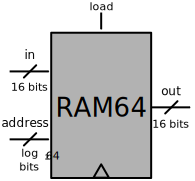
\includegraphics[width=0.3\textwidth]{imgs/ram-block.pdf}}
            \caption{Block diagram of circuit 2, a RAM of 64 lines
                \label{fig:ram-block}}
        \end{figure}

        The circuit has one 16-bit output, named \texttt{out}, and three inputs (\texttt{in},
        \texttt{address} and \texttt{load}). The \texttt{in} port is 16-bit wide and holds a value
        to be written into the RAM. The \texttt{address} port has a width of $\log_{2} 64 = 6$ bits
        and holds the address in which reading or writing is to be performed. Finally, the
        \texttt{load} bit controls whether the value currently at \texttt{in} should be written to
        the selected address. There is also one \emph{implicit} input for a clock signal in this
        component.  Implicit, in this case, means that the clock signal is not present in any of the
        models that we developed for this circuit, but must be present in any physical
        implementation.

        The temporal behaviour of this memory block is as follows: At any point in time, the output
        \texttt{out} holds the value stored at the memory location specified by \texttt{address}.
        If the \texttt{load} bit is high, then the value at \texttt{in} is loaded into the memory
        word specificied by \texttt{address}. The loaded value will then be emitted on the output at
        the \textbf{next} clock cycle.

    \subsection{Circuit 3: The Hack CPU}
    \label{subsec:hack-cpu-circuit}

        Circuit 3, the largest and most complex circuit among the ones we have chosen to implement,
        is the Central Processing Unit for the \emph{Hack} computer, the machine described in the
        book ``The Elements of Computing Systems''\cite{nand2tetris-book}.

        The Hack computer is based on the \emph{Harvard architecture}, that means that it has
        different storage components and signal pathways for instructions and data. Therefore, the
        Hack CPU expects to be connected to \emph{two} memory blocks, the instruction memory and the
        data memory. Having this in mind facilitates the understanding of the CPU's block diagram,
        shown in figure \ref{fig:cpu-block}

        \begin{figure}[H]
            \centerline{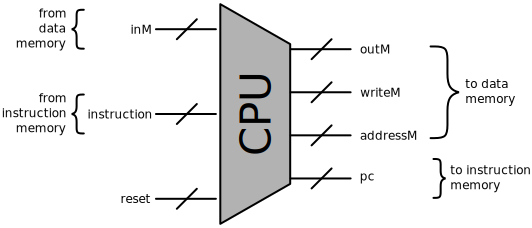
\includegraphics[width=0.85\textwidth]{imgs/cpu-block.pdf}}
            \caption{Block diagram of circuit 3, the Hack CPU
                \label{fig:cpu-block}}
        \end{figure}

        The Hack architecture has an \emph{extremely} reduced instruction set, and consists in fact
        of only two instructions (each 16-bit wide): A (meaning ``address'') and C (meaning
        ''compute''). The A instruction can be used as a means to load numerical literals into the
        data memory, as well as setting a special ``cache'' register inside the CPU. The C
        instruction is the one responsible for effectively performing computations using the ALU,
        testing outputs and jumping. More details about programming in the Hack assembly language
        can be found in \cite{nand2tetris-chapter-assembly}.

        The meaning of each of the CPU's input and output ports becomes much clearer when we look at
        the context in which the CPU is inserted, namely, the memory modules to which it is
        connected. So, let's analyze the CPU's ports by taking a look at figure
        \ref{fig:cpu-memory}.

        \begin{figure}[h!]
            \centerline{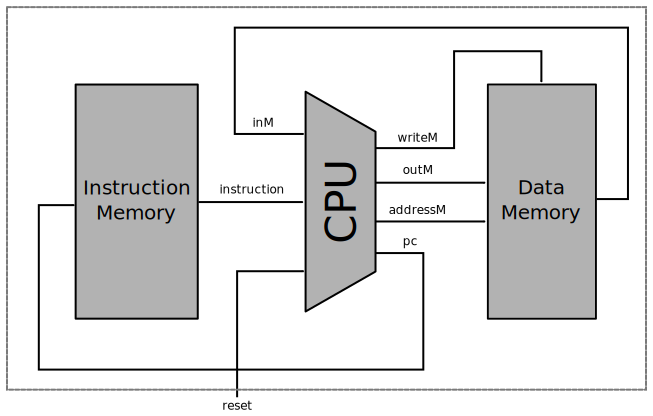
\includegraphics[width=0.85\textwidth]{imgs/cpu-memory.pdf}}
            \caption{The Hack CPU connected to the data and instruction memory blocks
                \label{fig:cpu-memory}}
        \end{figure}

        Finally, the CPU is a circuit which is built mostly from the parts we already defined in
        circuits 1 and 2. We use the ALU, some registers, multiplexers, an instruction decoder and a
        counter (the \emph{program counter}). Figure \ref{fig:cpu-parts} shows the CPU organization.

        \begin{figure}[h!]
            \centerline{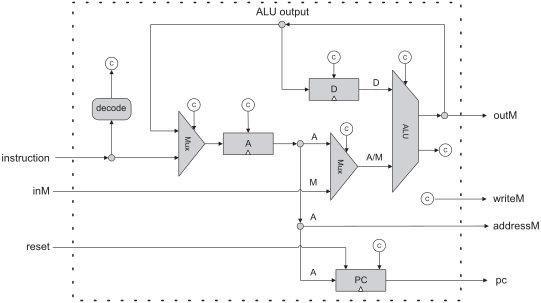
\includegraphics[width=1.0\textwidth]{imgs/cpu-parts.pdf}}
            \caption{Parts used in building the CPU circuit and how they are connected.
                \label{fig:cpu-parts}}
        \end{figure}

    \section{Analysis of the EDSLs}
\label{sec:analysis-of-the-edsls}
    \frame{\sectionpage}

    \subsection{Lava}
    \label{subsec:lava}
        % Lava intro
        \begin{frame}
            \frametitle{Lava}

            \begin{itemize}
                \item Developed at Chalmers University of Technology, Sweden
                    \begin{itemize}
                        \item Initially by Koen Claessen and Mary Sheeran
                        \item Later also Per Bjesse and David Sands
                    \end{itemize}

                \item Has several \emph{dialects}
                    \begin{itemize}
                        \item \texttt{chalmers-lava}, \texttt{xilinx-lava}, \texttt{kansas-lava}, etc. 
                        \item We focus on the ``canonical'' \texttt{chalmers-lava}
                    \end{itemize}
            \end{itemize}
        \end{frame}

        \begin{frame}
            \frametitle{Lava's \emph{key} characteristics}

            \begin{itemize}
                \item Deep-embedded
                \item Observable sharing
                    \begin{itemize}
                        \item ``Type-safe pointer equality'' to detect sharing and recursion
                        \item Advantages and disadvantages clearer with examples
                    \end{itemize}
                \item Capable of simulation, verification and synthesis
                    \begin{itemize}
                        \item Generates \emph{flat} VHDL
                        \item External tools for verification
                    \end{itemize}
                \item Very ``functional'' style of hardware description
                    \begin{itemize}
                        \item Will become clearer with examples
                    \end{itemize}
            \end{itemize}
        \end{frame}

        \begin{frame}
            \frametitle{Lava: Adders}
            \haskellfile{code/lava-adders.hs}
        \end{frame}

        \begin{frame}
            \frametitle{Lava: Simulation and verification}

            \begin{itemize}
                \item A taste of simulation in Lava:
                    \haskellfile{code/lava-simulation-halfadder.hs}
                    \begin{itemize}
                        \item Cannot be easily automated: equality of \texttt{Signal} is non-trivial
                    \end{itemize}

                \item And verification\ldots
                    \haskellfile{code/lava-verify-fulladder-comm.hs}
                    \begin{itemize}
                        \item Advantage: Used in conjunction with an external SAT solver (e.g. \emph{Satzoo})
                        \item Disadvantage: Only verifies instances of \emph{specific size}
                    \end{itemize}
            \end{itemize}
        \end{frame}

        % Lava ALU
        \begin{frame}
            \frametitle{Lava: ALU}
            \haskellfile{code/lava-alu.hs}
        \end{frame}

        \begin{frame}
            \frametitle{Remarks}

            \begin{itemize}
                \item Cannot introduce new, meaningful datatypes
                    \begin{itemize}
                        \item Only \texttt{Signal Bool} is synthesizable
                        \item Or tuples/lists thereof
                    \end{itemize}
                \item Input/Output types have to be \emph{uncurried}
                \item Weak type-safety over the inputs/outputs
                    \begin{itemize}
                        \item Working with tuples is tiresome and has limitations
                        \item Lists don't enforce \emph{size} constraints
                    \end{itemize}
            \end{itemize}
        \end{frame}

        % Lava RAM64
        \begin{frame}
            \frametitle{Lava: RAM64}
            \haskellfile{code/lava-ram64.hs}
        \end{frame}

        \begin{frame}
            \frametitle{Remarks}

            \par{Positive:}
            \begin{itemize}
                \item Uses host language for binding (\texttt{let}/\texttt{where}) and recursion
                \item Uses host language for structural combinators
            \end{itemize}

            \par{Negative:}
            \begin{itemize}
                \item Again, weak type-safety of lists
                    \begin{itemize}
                        \item Extra \texttt{Int} parameter controls port \emph{sizes}
                    \end{itemize}
                \item \emph{No modularity} in the generated VHDL code.
            \end{itemize}
        \end{frame}

        % Lava CPU
        \begin{frame}
            \frametitle{Lava: \emph{Hack} CPU (some parts)}
            \haskellfile{code/lava-cpu.hs}
        \end{frame}

        \begin{frame}
            \frametitle{Remarks}

            \par{Could benefit from:}
            \begin{itemize}
                \item Fixed-length vectors
                    \begin{itemize}
                        \item ForSyDe-style or with type-level naturals in recent GHC.
                    \end{itemize}
                \item Slicing operators over vectors
                \item \emph{Synthesizable} user-defined datatypes
            \end{itemize}
        \end{frame}


    \subsection{ForSyDe}
    \label{subsec:forsyde}
        % ForSyDe intro
        \begin{frame}
            \frametitle{ForSyDe}

            \begin{itemize}
                \item Based on the ``Formal System Design'' approach
                    \begin{itemize}
                        \item Royal Institute of Technology - KTH, Sweden
                    \end{itemize}
                \item Available for Haskell and SystemC
                \item Has BOTH shallow and deep-embedded ``versions''
                    \begin{itemize}
                        \item Same library, subtle distinction
                        \item Will become clearer with examples
                    \end{itemize}
                \item \emph{Template Haskell} to express circuits with Haskell syntax
            \end{itemize}
        \end{frame}

        \begin{frame}
            \frametitle{ForSyDe's key concepts}

            \begin{itemize}
                \item Models of Computation (MoCs)
                    \begin{itemize}
                        \item We focus on the \emph{synchronous} MoC
                    \end{itemize}
                \item Processes
                    \begin{itemize}
                        \item A process belongs to a MoC
                        \item Built with a \emph{process constructor}
                    \end{itemize}
                \item Signals
                    \begin{itemize}
                        \item Connections among processes
                    \end{itemize}
            \end{itemize}
        \end{frame}

        \begin{frame}
            \frametitle{ForSyDe's key concepts}
            \begin{figure}[h!]
                \centerline{\includegraphics[width=0.8\textwidth]{imgs/forsyde-model.pdf}}
                \caption{Key concepts of the ForSyDe EDSL
                    \label{fig:forsyde-model}}
            \end{figure}
        \end{frame}

        % ForSyDe ALU non-synth
        \begin{frame}
            \frametitle{ForSyDe: ALU (non-synth)}
            \haskellfile{code/forsyde-alusim-slide1.hs}
        \end{frame}

        \begin{frame}
            \frametitle{ForSyDe: ALU (non-synth)}
            \haskellfile{code/forsyde-alusim-slide2.hs}
        \end{frame}

        \begin{frame}
            \frametitle{ForSyDe: synthesis restrictions}
            \par{Restrictions imposed on a model by ForSyDe so that it can be translated to VHDL:}
            \begin{itemize}
                \item ProcFun-related:
                    \begin{itemize}
                        \item Limited argument types (instances of \texttt{ProcType})
                        \item \texttt{Int}, \texttt{Int8}, \ldots, \texttt{Bool}, \texttt{Bit}
                        \item Enumerated types (deriving \texttt{Data} and \texttt{Lift})
                        \item Tuples and \texttt{FSVec}'s
                    \end{itemize}
                \item VHDL engine-related:
                    \begin{itemize}
                        \item No point-free notation
                        \item Single clause / no pattern matching
                        \item No \texttt{where} or \texttt{let} bindings
                    \end{itemize}
            \end{itemize}
        \end{frame}

        % ForSyDe ALU synth
        \begin{frame}
            \frametitle{ForSyDe: ALU (synthesizable)}
            \haskellfile{code/forsyde-alusyn-slide1.hs}
        \end{frame}

        \begin{frame}
            \frametitle{ForSyDe: ALU (synthesizable)}
            \haskellfile{code/forsyde-alusyn-slide2.hs}
        \end{frame}

        % ForSyDe Simulation

        % ForSyDe RAM64
        \begin{frame}
            \frametitle{ForSyDe: Muxes}
            \haskellfile{code/forsyde-muxes.hs}
        \end{frame}

        \begin{frame}
            \frametitle{Remarks}
            %% both advantage and disadvantage of ForSyDe
            \par{Positive:}
            \begin{itemize}
                \item Generated VHDL is very \emph{modular}
                    \begin{itemize}
                        \item One VHDL \emph{entity} per ForSyDe component
                        \item Good for tool integration
                    \end{itemize}
            \end{itemize}

            \par{Negative:}
            \begin{itemize}
                \item Interface ``conflicts'' caused by \texttt{FSVec} and process constructors
                    \begin{itemize}
                        \item ``zip-unzip'' pattern
                    \end{itemize}
            \end{itemize}
        \end{frame}

        \begin{frame}
            \frametitle{ForSyDe: RAM64}
            \haskellfile{code/forsyde-ram64.hs}
        \end{frame}

        \begin{frame}
            \frametitle{Remarks}

            \begin{itemize}
                \item Component \emph{instantiation}
                    \begin{itemize}
                        \item Introduces \emph{hierarchy} in the design
                        \item Influences generated VHDL
                    \end{itemize}
                \item \emph{Manual} name management
                    \begin{itemize}
                        \item Error-prone
                        \item Every process must have a \emph{unique} identifier
                        \item Already was a (lesser) issue with the muxes
                    \end{itemize}
            \end{itemize}
        \end{frame}

        % ForSyDe CPU
        \begin{frame}
            \frametitle{ForSyDe: \emph{Hack} CPU (part)}
            \haskellfile{code/forsyde-cpu-decoder.hs}
        \end{frame}


    \subsection{Coquet}
    \label{subsec:coquet}
        \begin{frame}
            \frametitle{The \texttt{Circuit} type}
            \coqfile{code/coquet-circuit-type.v}
        \end{frame}

        \begin{frame}
            \frametitle{Coquet}
            \coqfile{code/coquet-halfadder.v}
        \end{frame}

        \begin{frame}
            \frametitle{Coquet}
            \coqfile{code/coquet-fulladder.v}
        \end{frame}

        % Meaning relation
        \begin{frame}
            \frametitle{Coquet: Meaning relation}
            \coqfile{code/coquet-meaning-relation.v}
        \end{frame}

        % Specification definitions
        \begin{frame}
            \frametitle{Coquet: Specification}
            \coqfile{code/coquet-realise-implement.v}
        \end{frame}

        % Adder proof (1)
        \begin{frame}
            \frametitle{Coquet: Correctness proofs}
            \coqfile{code/coquet-halfadder-proof.v}
        \end{frame}

        % How to do proofs in Coquet (tac, etc)
        \begin{frame}
            \frametitle{Coquet: How to prove correctness}
            \coqfile{code/coquet-tac.v}
            % rinvert: invert derivation of meaning relation, following structure of circuit.
            % realise_all: use the Implement and Realise classes as hints to transform goals.
            % unreify_all: get rid of iso's
            % destruct all boolean, then proof by case analysis, not so important.
        \end{frame}
        % Adder proof (2)

    \section{Conclusions}
\label{sec:conclusions}

    The models and test cases that we developed, along with the verification we performed, gave us
    a better understanding of how the hardware \acp{EDSL} Lava, ForSyDe and Coquet compare to each other
    \emph{from the point of view of a hardware designer}. This practical experience, combined with
    knowledge of the ``inner workings'' of each \ac{EDSL} and their host language, allowed for an
    informed discussion of each language's strong points and weaknesses. The most significant
    findings of this practical evaluation, categorized by evaluated aspect, are summarized here.

    \paragraph{Depth of embedding}
        None of the three evaluated \acp{EDSL} lie at the \emph{extremes} of embedding depth. Lava can be
        said to be \emph{deeply embedded}, however, its \texttt{Signal} datatype collaborates with
        the host language runtime so that \emph{cyclic structures} in circuits can be modeled as
        \emph{recursion in the host language}. ForSyDe has \emph{both} deep and shallow modeling
        capabilities, even though we only studied the deep model. In fact, ForSyDe's hackage
        page\cite{website:forsyde-hackage} promises a future version in which deep and shallow
        modeling constructs will be in different packages. Coquet has the ``deepest'' modeling of
        all studied \acp{EDSL}, and \emph{avoids} the issue of \emph{observable sharing} by not allowing
        variable binding constructs, and having circuits connect to each other only through
        combinators.

    \paragraph{Simulation}
        Simulation can be performed in all studied \acp{EDSL}. In Lava, \emph{automated} test cases
        (in which the simulation output is compared with an \emph{expected} combination) are not
        possible due to the way in which the observable sharing issue is handled. Coquet has
        simulation built into the library as one of several \emph{example interpretations} for
        circuits, and it works just as well as in the other \acp{EDSL}, with the only shortcoming
        that simulation of \emph{sequential} circuits is currently \emph{not possible}.

    \paragraph{Verification}
        ForSyDe offers no capabilities for formal verification whatsoever, while Lava and Coquet
        each do, but in different ways. Lava can perform the verification of so-called \emph{safety
        properties} for circuits of a fixed size -- it does this by transforming the circuit model
        into a CNF (\emph{conjunctive normal form}) logical formula which is fed into a
        satisfiability solver. Coquet takes a different approach and offers some tools to help the
        user perform \emph{interactive theorem proving} for circuit correctness. One can say that
        Coquet does \emph{more than verification}, as with Coquet we can prove the correctness of
        whole families of parameterized circuits by induction.

    \paragraph{Genericity}
        In Lava the modeling of generic circuits is made very easy, and any parameter to a circuit
        definition which is not of type \texttt{Signal T} is considered a \emph{parameter} instead
        of a circuit input, and specific instances of these generic circuits can then be simulated
        or synthesized. In Coquet a similar approach is taken, allowing the user to prove \emph{by
        induction on the parameter} the correctness of the whole family of circuits.  ForSyDe is the
        \ac{EDSL} with the least opportunity for generalization: the only thing we can do is to have
        fixed-length bit vectors or fixed-size integers as inputs, and these are fixed at
        \emph{Haskell compilation time}.

    \paragraph{Tool integration}
        Lava can generate VHDL netlists of circuit models that satisfy some requirements and can
        also generate CNF formulas for a SAT solver. ForSyDe can output its circuits in VHDL and
        also generate \emph{graph files}, which can be formatted and used for circuit visualization.
        Coquet is disadvantaged when it comes to tool integration: it currently has no support for
        exporting circuits in some industry-standard format, even though one of the examples in the
        distribution is a gate-count, so netlist generation should be possible in the same
        framework.

    \paragraph{Extensibility}
        ForSyDe and Coquet offer both good capabilities for extensibility: in both \acp{EDSL} the
        designer can make circuits operate over user-defined types. The big advantage of ForSyDe is
        its usage of Template Haskell and GHC's \emph{deriving} mechanism to generate VHDL
        corresponding to the user-defined types. Lava offers little to no extensibility, and only
        circuits operating on booleans or integers can be modeled in the current version of Chalmers
        Lava.



\end{document}
